\section{Experiment Results}

We now evaluate the NetLearner-implemented model on the 5-class NSL-KDD task,
as well as on the 2-class UNSW-NB15 task, using the following metrics.
\begin{itemize}
    \item \textbf{Accuracy} is the percentage of correctly classified connections
        over the total number of connections in the dataset:
        \begin{align}
            A = \frac{\text{Correct Predictions}}{\text{Number of Records}}
        \end{align} 
        Accuracy is not suitable for evaluating biased dataset where the number
        of records of some class is extremely larger than the number of
        records of another class.
        In NSL-KDD dataset, the number of available U2R records (67)
        is in two degrees of magnitude less than the other classes of traffic
        (9711, 7458, 2887, 2121 respectively).
        Therefore we also consider the precision and recall.
    \item \textbf{Precision} is the percentage of the correctly classified positives over
        the total number of positives predicted by the classifier:
                \begin{align}
                    P = \frac{\text{True Positives}}{\text{True Positives} + \text{False Positives}}
                \end{align}
    \item \textbf{Recall} is the percentage of the correctly classified positives over
        the total number of relevant elements:
                \begin{align}
                    R = \frac{\text{True Positives}}{\text{True Positives} + \text{False Negatives}}
                \end{align}
    \item \textbf{F1-Score} represents a balance between precision and recall and is calculated
        as their harmonic mean:
                \begin{align}
                    F = \frac{2PR}{P + R}
                \end{align}
\end{itemize}
%In the 5-class classification, we calculate the precision, recall and F1-Score for each traffic class.
%Additionally, we report the weighted average of these metrics as a single value for comparing various approaches.
%The weight for each class is determined by its proportion in the test dataset.
%The weight vector for class [Normal, Probe, DoS, U2R, R2L] is [0.431, 0.107, 0.339, 0.018, 0.105].

Besides, we also calculate the confusion matrices of the classification results when applying
different approaches on both task's test datasets.
In a confusion matrix table, the $i$th row represents the instances of class $i$,
while the $j$th column represents the instances predicted by the classifier as class $j$.
It is called confusion matrix because it is useful for visualizing how a classifier
is confusing one class with other classes.
Due to page space limit, here we only present the most straightforward
and relatively more important metric accuracy.
Statistics regarding precision, recall and confusion matrices can be found
in our detailed technical report~\cite{OurWonReport} and our codebase~\cite{NetLearner}.

For comparison, we train a SVM using~\cite{ScikitLearnSVM} and report its accuracy along
with multilayer perceptron (MLP), finetuned restricted Boltzmann machine (RBM),
finetuned sparse autoencoder (SAE) and wide and deep combined model (WnD).
Since the weights in neural networks are usually initialized randomly, we repeat forty
runs (training and testing) for each model and plot the mean accuracies and their standard deviation.
The training and testing results for 5-class NSL-KDD task and 2-class UNSW-NB15 task are
shown in Figure~\ref{Fig:CompAccuracyNSL} and Figure~\ref{Fig:CompAccuracyUNSW} respectively.


\begin{figure}[h]
    \centering
    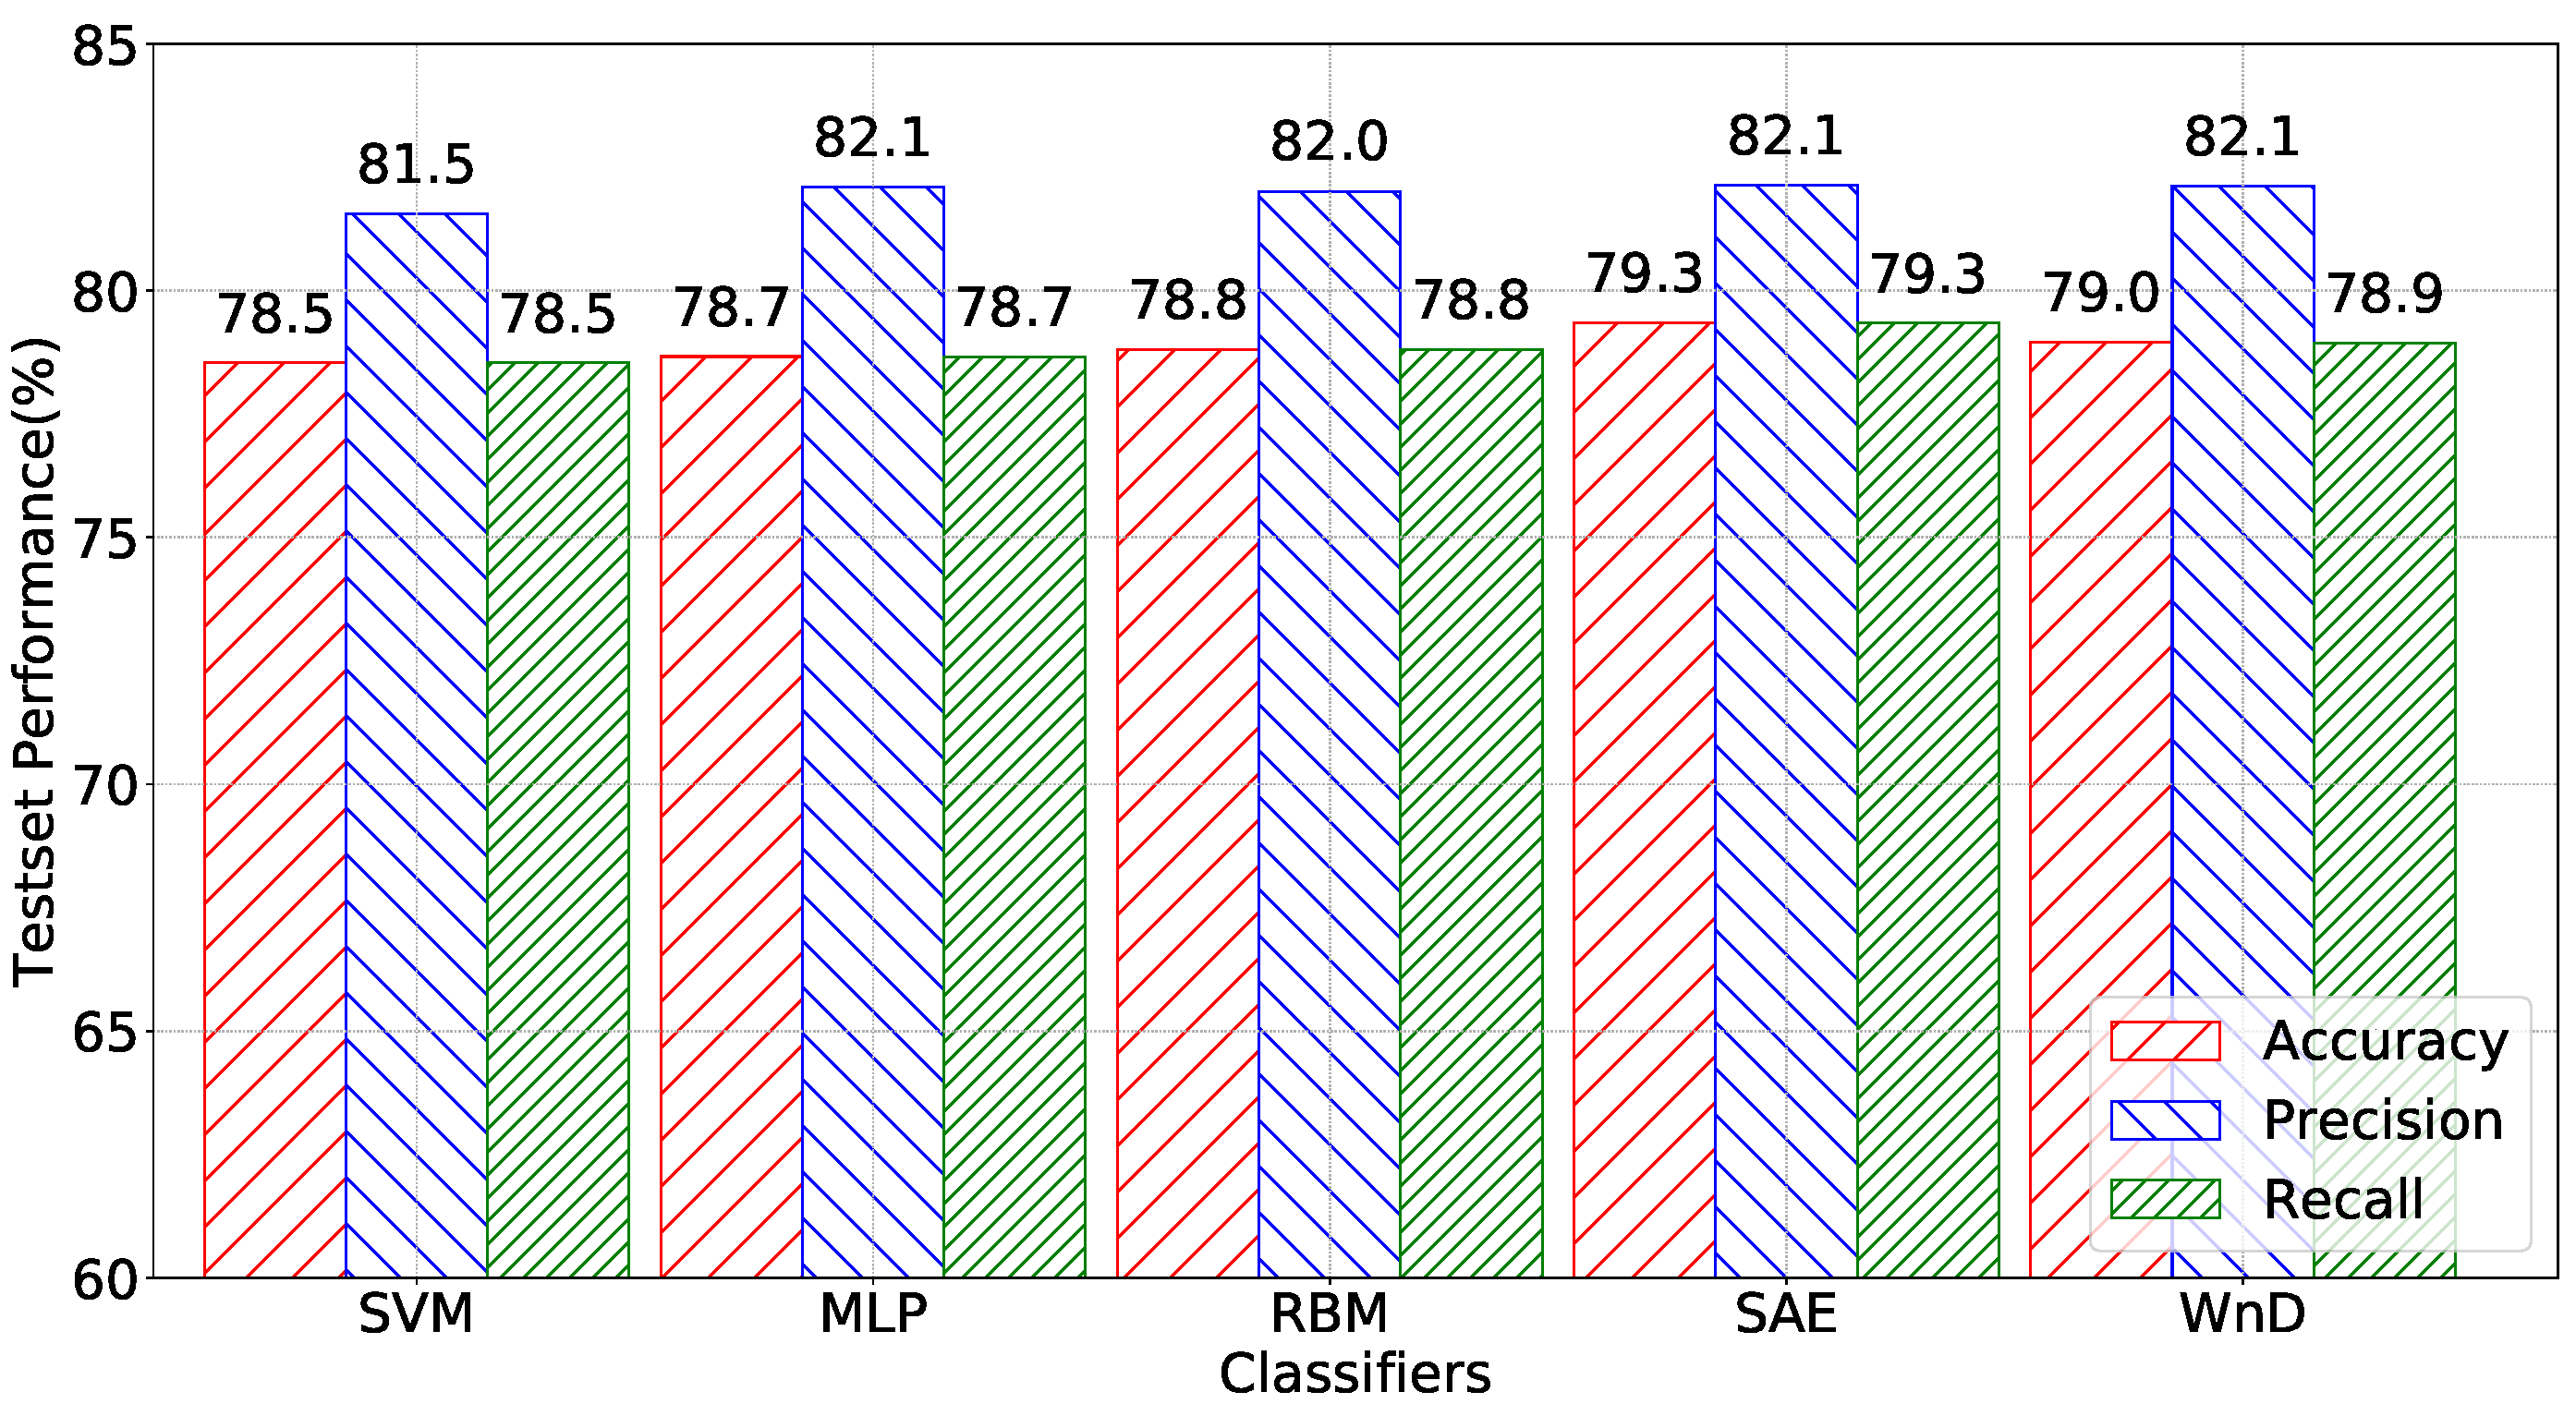
\includegraphics[width=0.48\textwidth]{figures/comp_accuracy_nsl.pdf}
    \caption{Classification Accuracy of Proposed Approaches on NSL-KDD Dataset}
    \label{Fig:CompAccuracyNSL}
\end{figure}

\begin{figure}[h]
    \centering
    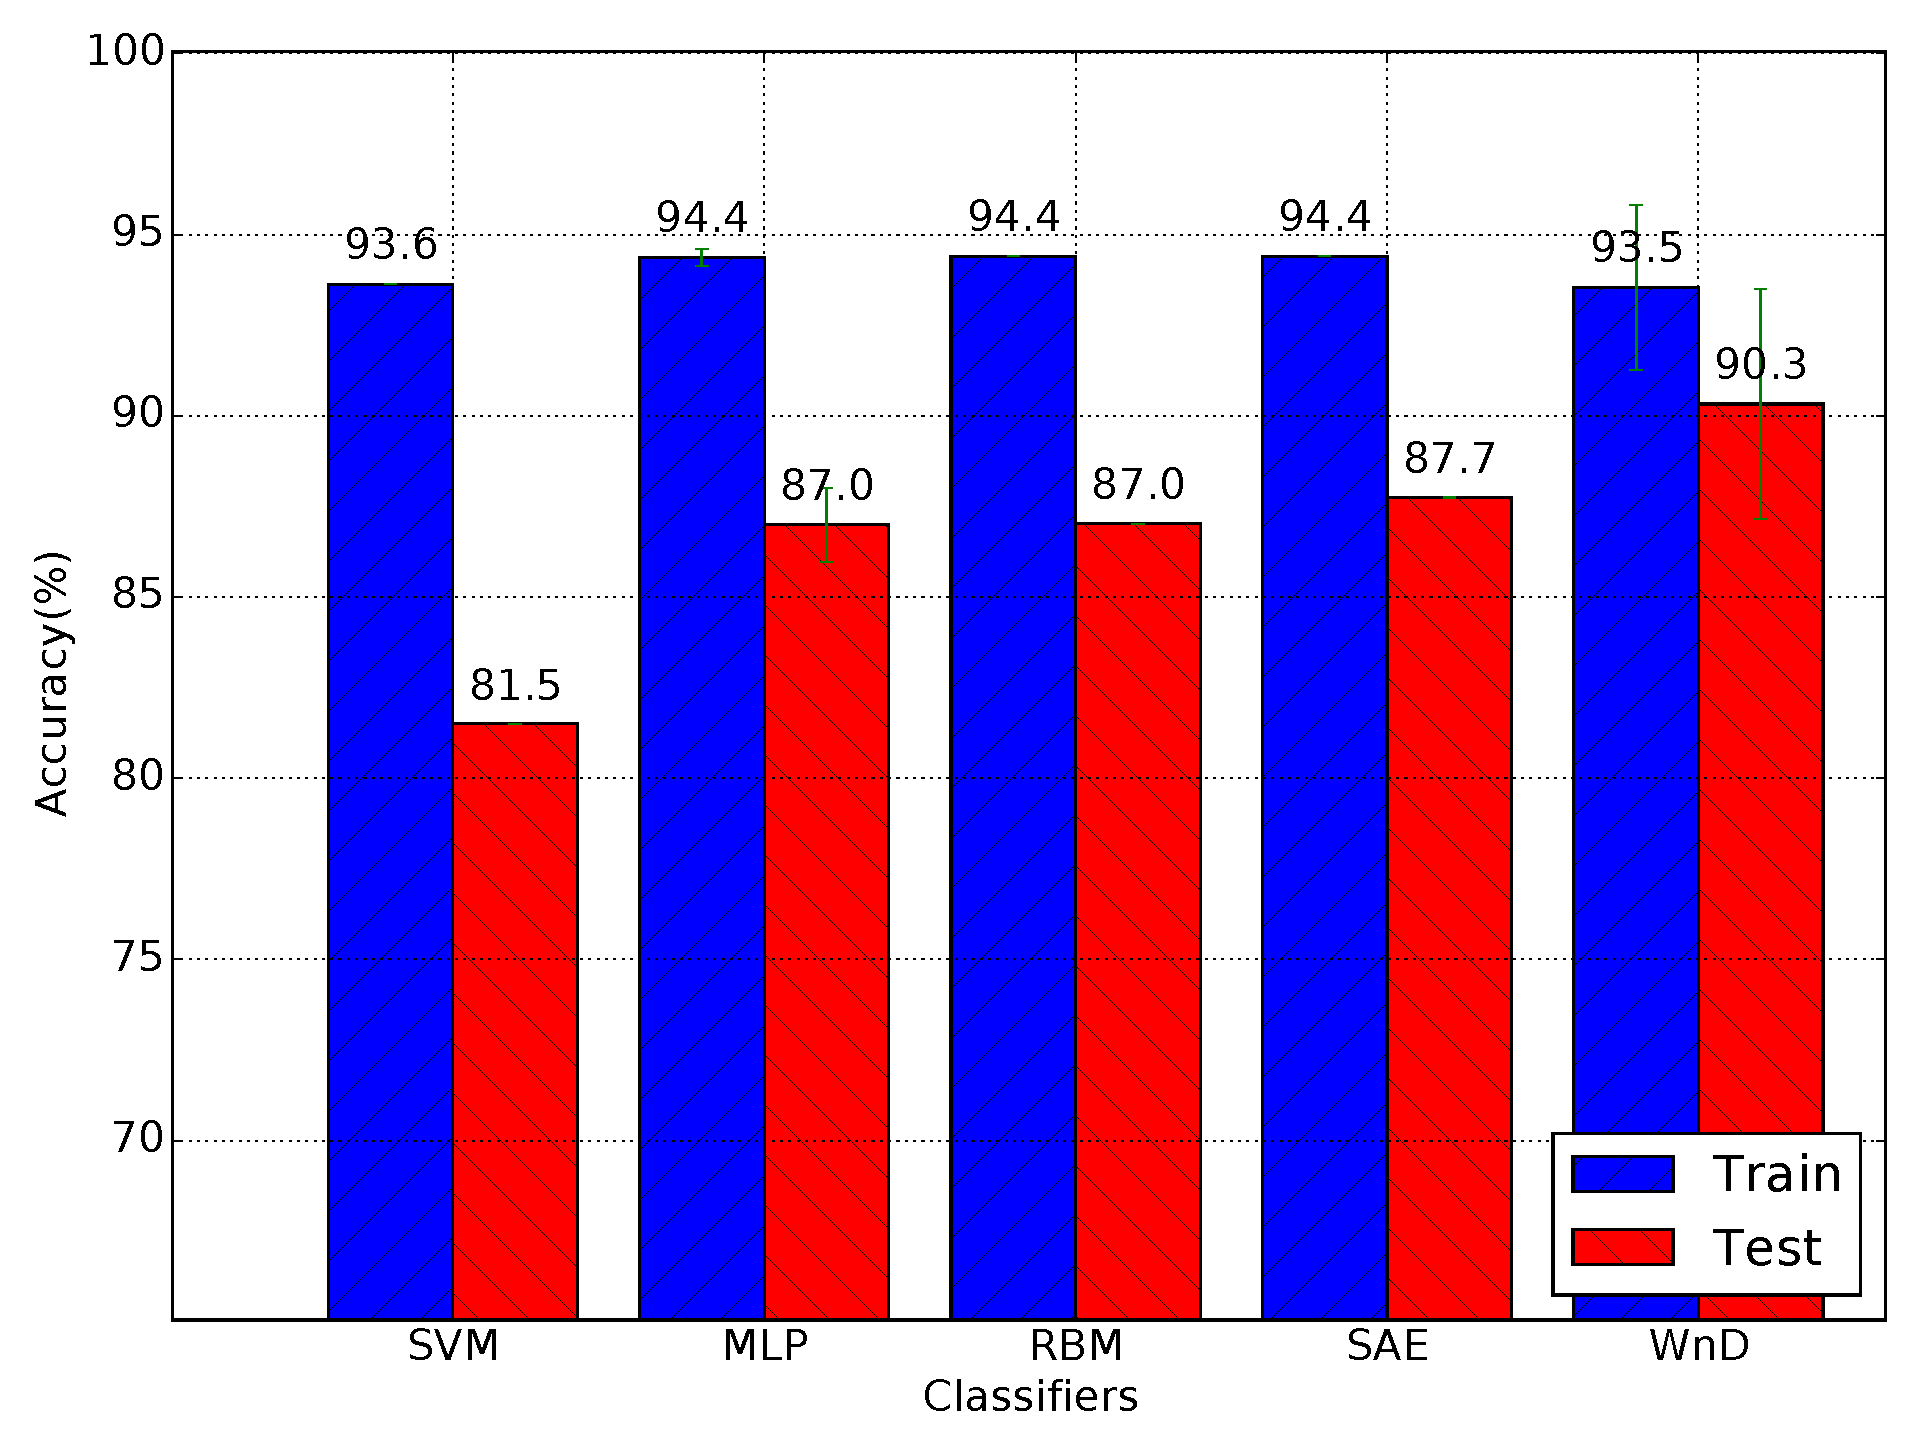
\includegraphics[width=0.48\textwidth]{figures/comp_accuracy_unsw.pdf}
    \caption{Classification Accuracy of Proposed Approaches on UNSW-NB15 Dataset}
    \label{Fig:CompAccuracyUNSW}
\end{figure}

